\documentclass{article}


\usepackage[final]{neurips_2024}



\usepackage[utf8]{inputenc} % allow utf-8 input
\usepackage[T1]{fontenc}    % use 8-bit T1 fonts
\usepackage[hidelinks]{hyperref}       % hyperlinks
\usepackage{url}            % simple URL typesetting
\usepackage{booktabs}       % professional-quality tables
\usepackage{amsfonts}       % blackboard math symbols
\usepackage{nicefrac}       % compact symbols for 1/2, etc.
\usepackage{microtype}      % microtypography
\usepackage{xcolor}         % colors
\usepackage{graphicx}

\title{A MARL Approach to IoT Sensor Charging Efficiency via RF Energy Harvesting and Directional Antennas}

\author{
  Yu-Hsiu Hung  \\
  Department of Computer Science\\
  National Tsing Hua University\\
  Hsinchu, Taiwan \\
  \texttt{elison8934678@gmail.com} \\
}


\begin{document}


\maketitle


\begin{abstract}
The IoT sensors possess monitoring and computational functions, interconnected through a network. However, data transmission depletes battery energy. To sustain sensor operation, charging is typically done using radio frequency (RF) energy. These energy sources, equipped with directional antennas and utilizing energy harvesting technology to charge the sensors, need to cooperate to keep the sensors in the environment operational. In practical applications, the efficiency of energy transmission is affected by the distance between the energy sources and the sensors, a concept known as path loss. Considering the above factors, I constructed a simulation environment and modeled it as a full-cooperative decentralized partially observable Markov decision process (Dec-POMDP) problem. I implemented multi-agent reinforcement learning (MARL) algorithms to provide a decentralized control system to manage the energy sources with directional antennas, aiming for optimal charging efficiency. I compared the performance of QMIX and Independent Q-learning (IQL) on this problem and analyzed the reasons behind the experimental results. Source codes is available at \href{https://github.com/Forcer0625/DRL-Final}{https://github.com/Forcer0625/DRL-Final}.
\end{abstract}


\section{Introduction}


Today, IoT technology has been applied across various industrial systems. Sensors, which possess monitoring and computational capabilities, are interconnected through networks. However, data transmission inevitably depletes the device's battery energy. In most cases, replacing sensor batteries is impractical due to high costs. Consequently, maintaining sensor operation using radio frequency (RF) energy has become a common solution. Energy sources for charging sensors are generally categorized into two types: omnidirectional and directional antennas. While the range of directional antennas is limited, they concentrate energy more efficiently, making them the focus of this research.

Energy harvesting refers to the technology of collecting and converting small amounts of energy from the surrounding environment to power sensors. These energy sources can include solar, thermal, kinetic, and radio frequency energy. This technology plays a significant role in reducing dependency on traditional batteries and enabling the continuous operation of wireless sensor networks and IoT devices.

The distance between the energy source and the sensor also affects the efficiency of energy transmission, a concept known as path loss. The greater the distance between the energy source and the sensor, the less energy the sensor receives.

Given the above description, multiple energy sources must cooperate to charge sensors distributed throughout the environment. They share a common goal and need to control the direction of their directional antennas to emit RF energy under limited communication conditions. Therefore, this environment can be modeled as a full-cooperative decentralized partially observable Markov decision process (Dec-POMDP) \cite{oliehoek2016concise}.

Multi-agent reinforcement learning (MARL) has shown significant performance in solving Dec-POMDP problems. In MARL, each agent learns an optimal policy through interactions with the environment and other agents to achieve a common goal. In the context of wireless charging, each energy source acts as an agent, learning to collaborate under limited communication to maximize the energy harvesting efficiency of the sensors.

Centralized training and decentralized execution (CTDE) is a widely used framework in MARL. CTDE allows for the collection of all agents' state and action information during training to more efficiently learn cooperative strategies. During execution, each agent makes decisions independently based on its local observations. This approach is particularly effective in systems requiring decentralized control, making it suitable for multi-energy sources control problems in wireless sensor networks.

\section{Related Works}
\cite{ko2018phase} proposed a model similar to the one in this paper, where multiple energy sources charge sensors within a certain range. However, there are some key differences. In the model, the sensors are divided into several sectors, and each charging operation fully charges all sensors within a sector, without considering the distance and actual location of the sensors. Additionally, the model features a controller that directs the antenna of all energy sources, functioning as a centralized control system. As a result, the energy sources cannot make optimal decisions based solely on their own conditions, making this model unsuitable for scenarios with communication constraints or where low latency is required.

Independent Q-learning (IQL) \cite{tan1993multi} is the simplest and most straightforward approach, but it does not account for the interactions between agents, and its convergence cannot be guaranteed. Despite this, it often performs well in practice \cite{tampuu2017multiagent}.

QMIX \cite{rashid2020monotonic} is a MARL algorithm designed for multi-agent systems to address cooperative problems within the CTDE framework. It decomposes the original problem's state-action value into a weighted sum of individual agents' state-action values through a mixing network, optimizing the cooperative objective while retaining the decentralized execution capability of individual agents.

QMIX is trained end-to-end with the objective of minimizing the following loss:
\begin{equation}\label{loss}
Loss={1\over B}\sum\Big(y^{tot}-Q_{tot}(s^{t},a^t;\theta)\Big)^2,
\end{equation}
where $B$ represents the batch size sampled from the replay buffer, $y^{tot} = \normalsize r^t+\gamma \mathop{\max}\limits_{a'}Q_{tot}(s^{t+1},a';\bar\theta)$, and $\bar\theta$ denotes the parameters of a target network as in DQN \cite{mnih2013playing}.

\section{Multiple Energy Sources and Harvesting Model}


\subsection{Environment}

At initialization, all sensors start with zero battery energy and are randomly distributed within a circle of radius $L$, with a total of $S$ sensors in the environment.

The distribution of energy sources (e.g., agents) follows a normal distribution with a mean of $L/2$ and a standard deviation of $L/8$. As the number of energy sources $N$ varies, their distribution forms a regular $N$-polygon, as shown in Figure \ref{Agent_Distribution}, to ensure even coverage of sensors throughout the environment. The darker areas indicate higher probability densities. In the experiment, $L$ is set to $500$ meters, meaning sensors and energy sources are distributed within a $500$-meter radius. The experimental setup includes $N=3$ energy sources and $S=10$ sensors.

\begin{figure}[htb]
	\centerline{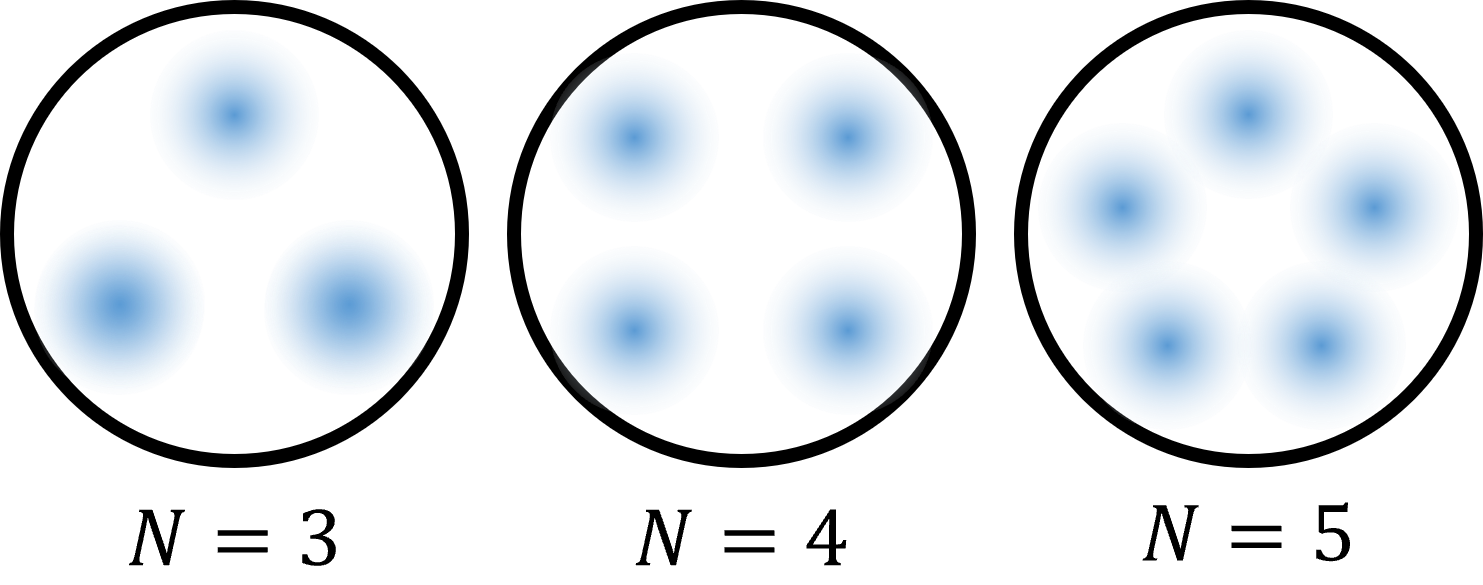
\includegraphics{Agent_Distribution.png}}
	\caption{Agents Distribution}\label{Agent_Distribution}
\end{figure}

At each time step $t$, all agents decide the direction of their antenna, $\phi_i^t$, based on their observation $o_i^t$. The observation $o_i^t$ includes the positions of the agent to the center of the circle, the coordinates of other energy sources, the sensors relative to itself and the current battery levels. The global state $s^t$ comprises the absolute coordinates of all energy sources and sensors, the current angles of the energy sources, and the battery levels of the sensors; this global state is used only by the QMIX algorithm. The direction of the directional antenna is determined by a mapping relationship in Equation \ref{phiti} to align with MARL algorithms like QMIX and IQL, which are designed for discrete action spaces. The emission angle, centered on the agent, ranges from $0$ to $2\pi$, with $A$ denoting the number of possible actions. In the experiment, $A$ is set to $32$.

\begin{equation}\label{phiti}
\phi^t_i = 2\pi{a_i^t\over A}
\end{equation}

The emission angle determines the agent's energy transmission range, covering the angle from $\phi_i^t-\phi_w$ to $\phi_i^t+\phi_w$, where only sensors within this range can be charged through energy harvesting, as illustrated in Figure \ref{Coverage}. In the simulation, $\phi_w$ is set to $\pi/8$.

\begin{figure}[htb]
	\centerline{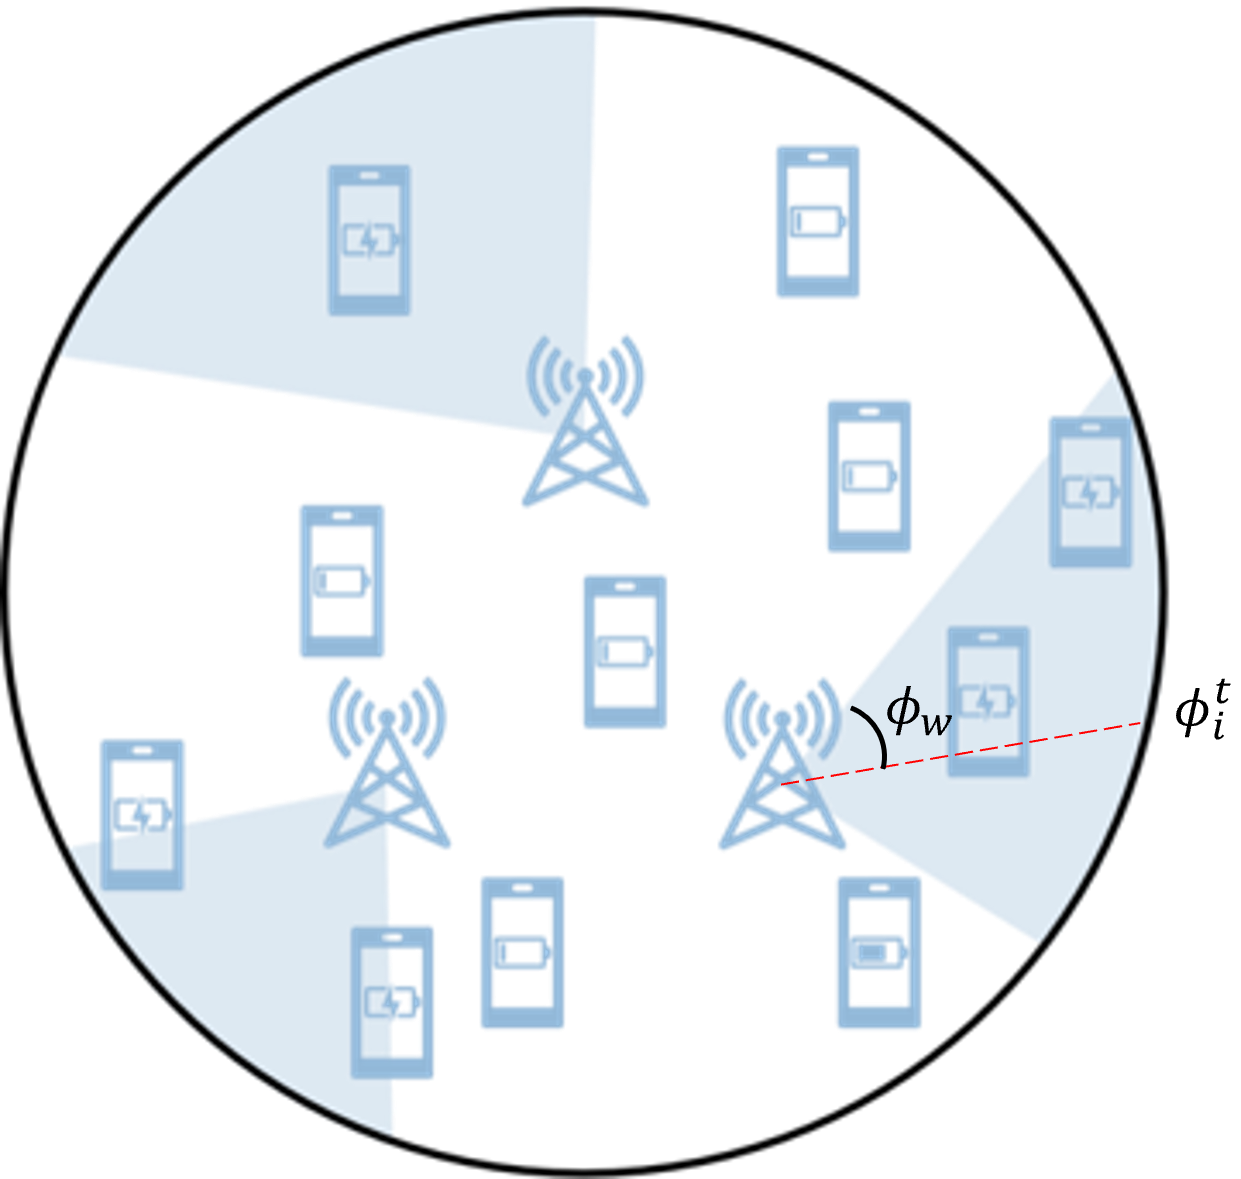
\includegraphics[width=0.4\linewidth]{Coverage.png}}
	\caption{Coverage of Sensors}\label{Coverage}
\end{figure}

The reward function is defined such that for each sensor whose battery level reaches 100\%, a reward of $1$ is given. The environment resets either when all sensors are fully charged or when the time limit is exceeded, defining an episode. The maximum number of steps per episode is set to $T=50$. Additionally, to encourage agents to charge the sensors as quickly as possible, a default penalty of $-0.1$ is applied at each time step.


\subsection{Path Loss}

The energy transmitted ($P_t$) by the energy source and the energy actually received ($P_r$) by the sensor are related as shown in Equation \ref{path_loss}. This formula is derived from the literature \cite{wang2017transmission}. Here, $\phi_w$ represents the angle covered by the energy source; $\phi_s$ is the reception angle of the sensor, set to $2\pi$, indicating that the sensor can receive energy from any energy source. The path loss exponent $\alpha$ typically ranges between $2$ and $6$ \cite{rappaport2024wireless}; based on the settings in \cite{zhang2015optimal}, $\alpha$ is set to $3$. The variable $d$ denotes the straight-line distance between the target sensor and the energy source.

\begin{equation}\label{path_loss}
{P_r\over P_t}=\big(\normalsize {4\pi^2\over \phi_w\phi_s}\big)\times d^{-\alpha}
\end{equation}

\section{Result}
Figure \ref{result} presents the average results of 10 independent training runs for each method. The horizontal axis represents time steps, while the vertical axis denotes episode reward. Table \ref{parameters} details the training parameters.
\begin{figure}[htb]
	\centerline{\includegraphics[width=0.6\linewidth]{result.png}}
	\caption{Result}\label{result}
\end{figure}
The MARL algorithm demonstrates effective performance in addressing this problem: within the environment, there are 10 sensors, and fully charging all of them yields a total reward of 10. Considering a penalty of -0.1 over a maximum of 50 steps, the expected reward hovers around 5. If charging can be completed earlier, the reward will exceed 5.

Additionally, the comparison between the two algorithms reveals that QMIX outperforms IQL, which relies solely on local observations. I attribute this superior performance to the advantages provided by CTDE. This demonstrates that leveraging centralized information during training can significantly enhance performance. The centralized approach in QMIX allows for more informed decision-making by incorporating global state information, which is not accessible to individual agents in IQL. Consequently, this centralized strategy during training results in more efficient coordination and improved overall outcomes in multi-agent environments.

\begin{table}[htb]
    \caption{Hyperparameters}\label{parameters}
\begin{tabular}[c]{|l|c|}
    \hline
    \textbf{Parameters} & \textbf{Value}\\
    \hline
    optimizer &  Adam \\
    \hline
    learning rate & $10^{-4}$\\
    \hline
    discount factor & $0.99$\\
    \hline
    replay buffer size & $10^6$\\
    \hline
    number of hidden layers (all network) & $2$\\
    \hline
    number of hidden units per layer & $128$\\
    \hline
    number of hidden units per layer (mixing network) & $64$\\
    \hline
    number of samples per minibatch & $256$\\
    \hline
    nonlinearity & ReLU\\
    \hline
    target smoothing coefficient & $0.005$\\
    \hline
    target update interval & $1$\\
    \hline
\end{tabular}\centering
\end{table}

{
\small
\bibliographystyle{unsrt}
\bibliography{reference}
}



\end{document}